%\documentclass[draft]{chi2009}
%\documentclass[draft]{sigchi}
\documentclass{sigchi}

\usepackage{times}
\usepackage{url}
%\usepackage{graphics}
\usepackage{color}
\usepackage[usenames,dvipsnames]{xcolor}
\usepackage{blindtext}
\usepackage[ddmmyyyy]{datetime}

\usepackage{graphicx}

\usepackage{float}

\widowpenalty=10000
\clubpenalty=10000

\newcommand{\comment}[1]{\footnote{DELETED FOR NOW -- \textcolor{Shadow}{#1}}}
\newcommand{\killedForSpace}[1]{}
\newcommand{\kfs}[1]{}

\definecolor{Orange}{rgb}{1,0.5,0}
\definecolor{Shadow}{rgb}{0.1,0.1,0.1}
\definecolor{Shadowy}{rgb}{0.2,0.2,0.2}
\definecolor{Purple}{RGB}{75,0,130}
\definecolor{LightBlue}{RGB}{135,206,250}
\definecolor{Blueish}{RGB}{30,144,255}
\newcommand{\todo}[1]{\textrm{\textbf{\textcolor{Purple}{[[#1]]}}}}
\newcommand{\todolater}[1]{}
\newcommand{\remove}[1]{}
%\newcommand{\remove}[1]{\textrm{\textbf{\textcolor{Salmon}{[[#1]]}}}}
\newcommand{\rephrase}[1]{\textrm{\textrm{\textcolor{Blue}{[[#1]]}}}}
\newcommand{\rewrite}[1]{\textrm{\textrm{\textcolor{Gray}{[[#1]]}}}}
\newcommand{\revised}[1]{{\textrm{\textrm{\textcolor{Purple}{[[#1]]}}}}}
%\newcommand{\revision}[1]{\textrm{\textrm{\textcolor{LightBlue}{#1}}}}
%\newcommand{\qq}[2]{\textrm{\textit{\textcolor{Shadow}{``#2''}}}}
\newcommand{\qq}[2]{\textrm{\textit{``#2''}}}

%{{{ Initial definitions
\iffalse
\usepackage[abbr]{harvard}
\harvardparenthesis{none}
\harvardyearparenthesis{round}
\citationstyle{dcu}
\fi

%\emergencystretch=1em

%\pagenumbering{arabic}  % Arabic page numbers for submission.  Remove this line to eliminate page numbers for the camera ready copy

\begin{document}
% to make various LaTeX processors do the right thing with page size
\special{papersize=8.5in,11in}
\setlength{\paperheight}{11in}
\setlength{\paperwidth}{8.5in}
\setlength{\pdfpageheight}{\paperheight}
\setlength{\pdfpagewidth}{\paperwidth}

% use this command to override the default ACM copyright statement
% (e.g. for preprints). Remove for camera ready copy.
%\toappear{Submitted for review to CHI 2009.}
\toappear{
Permission to make digital or hard copies of all or part of this work for personal or classroom use is granted without fee provided that copies are not made or distributed for profit or commercial advantage and that copies bear this notice and the full citation on the first page. To copy otherwise, or republish, to post on servers or to redistribute to lists, requires prior specific permission and/or a fee.\\
{\confname{CSCW'14}}, \\
Copyright 2013 ACM 978-1-XXXX-XXXX-X/XX/XX...\$10.00. }

\title{On Becoming a Counsellor: Challenges and Opportunities To Support Interpersonal Skills Training}
\numberofauthors{1}
% blinded authors
\iffalse
\author{
  \alignauthor Petr Slov\'{a}k$^{1}$, Anja Thieme, Paul Tennent, Patrick Olivier, Geraldine Fitzpatrick$^{1}$ \\
      \affaddr{$^1$Human Computer Interaction Group, Vienna University of Technology, Austria}\\
      \affaddr{$^2$Culture Lab, University of Newcastle, UK} \\
      \affaddr{$^3$Mixed Reality Laboratory, University of Nottingham, UK} \\
    % \email{\{petr,geraldine.fitzpatrick\}@igw.tuwien.ac.at, paul.tennent@nottingham.ac.uk}
}	
\fi	


\author{
  \alignauthor ~\\
      \affaddr{~}\\
      \affaddr{~}\\
      \affaddr{~}
}

\maketitle
%}}}

% {{{ Abstract
\begin{abstract}
Well-developed interpersonal skills are crucial for all social interactions. However, understanding how interpersonal skills are taught or learned, and how technology can play a part in this, is yet an under-researched area in CSCW and HCI research. 
%
To start addressing this gap, our research explores the learning processes of counselling students, for whom developing interpersonal skills forms a fundamental part of their university education. We followed an iterative process to gain an in-depth understanding of this context, combining interviews and low-fidelity technology prompts. Overall, 26 participants comprising tutors, students and expert counsellors took part. 
%
Our findings first provide insights into the highly collaborative and social learning process of the students. We highlight the complexity of interpersonal reflection as a crucial process for developing counselling skills, and identify the challenges to learning that students face. Second, we build on this understanding to draw out empirically grounded design considerations around opportunities for technology innovation in this setting.
\end{abstract}


\section{Author Keywords}
Relational Skills; Empathy; Education; Healthcare; Counselling Training; Reflective Design. 

\section{ACM Classification Keywords}
H.5.m. [Information interfaces and presentation]: Miscellaneous.
% }}}


%%% STUDENT LABEL CODE: 
% S2 -> S6
% Julie -> S12
% Ben -> S15
% Lily == S1
% Carolyn -> S11



% {{{ SECTION: Introduction
\section{Introduction}

The importance of interpersonal skills in our everyday lives has been widely acknowledged \cite{Cohen2006,Kennedy2011,Durlak2011,Hill2006,Stepien2006}. Interpersonal skills are particularly important for mental health professionals such as counsellors and psychotherapists. Indeed, it is the counsellors' interpersonal skill and competence---gained through education, training, and experience---that is considered one of the critical elements for the positive effects of counselling interventions \cite[p.29]{Duncan2010}. However, thus far, no research has yet explored how digital technology could support counselling education, and the interpersonal skills training of students. 
%the role that digital technology could play in counselling education, or how students could be supported by technology in developing their interpersonal skills.

As a first step in this direction, this paper focuses on counselling students, for whom interpersonal skills development forms a crucial part of their university education and who have access to established training programs to support them in the learning of such skills. 
Our research aims to reach a deep understanding of the processes and challenges of how interpersonal skills are taught and learned in counselling; to outline opportunities for technology support; and to offer specific examples of how some of these may translate into technology design.

In the rest of this paper, we report on a study with students and tutors of an under- and postgraduate  counselling program at a leading university in the UK over a period of 14 months. We use an iterative process based on a series of interviews and observations (see Table 1 for an overview), with the later phases including low-fidelity prototypes that were employed to deepen discussions with participants and to enhance both their and our understanding of opportunities for technology design in this setting.

We begin with a review of related work and describe how technology has been previously employed for supporting interpersonal skills learning in other settings. Following a description of our iterative research and design process, our findings are then presented in three parts. The first describes the fundamental learning practices in counselling training. We particularly focus on the use of experiential and non-directive learning, and the importance of \emph{interpersonal reflection} in the learning process. Drawing on this understanding, the second part then describes the \emph{key challenges to learning} in this context and identifies a set of four \emph{design considerations} for supporting counselling skills by technology. These include opportunities for (i) non-directively promoting students' reflection processes; (ii) helping in the co-construction of interpersonal interpretation; (iii) scaffolding constructive feedback; and (iv) facilitating iterative, multi-phase reflection over time. In part three, we build on these considerations to guide the development of a design prompt used to further explore and deepen our understanding of the identified challenges and the possible design directions. We conclude by highlighting the complementarity of the interpersonal reflection process with previous works on reflection within CSCW and HCI communities. 

This paper makes two important contributions. First, we provide a nuanced understanding of how interpersonal skills are taught in this particular counselling setting, and outline the related challenges learners face. Second, we provide empirically driven design considerations for systems to address some of these challenges, and support the learning of interpersonal skills more generally. In doing so, this paper introduces a novel research context for supporting the learning of interpersonal skills, arguing that this is an important but so far under-researched area in CSCW, with wider implications for other contexts in which social and emotional skills learning is relevant.
% }}}

% {{{ SECTION: Background
\section{Background}
\subsection{Counselling skills and education}
Counselling is part of the psychotherapy profession, with several competing schools of thought that differ in the approach to client and philosophical background (cf. \cite{Coyle2007}). Interpersonal skills such as the abilities to deeply understand the other, give attention, reflect, listen, or paraphrase, are however at the core of counsellors' training, regardless of the chosen school or training model. In addition, humanistically oriented training such as the counselling program that was the focus of our research, emphasizes the Rogers' three core conditions of a therapist \cite{Rogers1980}. First is \emph{deep empathic understanding}, when the therapist is `so much inside the private world of the other that he or she can clarify not only the meanings of which the client is aware but even those just below the level of awareness'. The second is \emph{unconditional positive regard}, during which the therapist experiences a `positive, acceptant attitude toward whatever the client is at that moment', i.e, accepts the client without judgment or conditions. Finally, \emph{congruence} points to a `close matching between what is being experienced at the gut level, what is present in counsellor's awareness, and what is expressed to the client', i.e., full authenticity of the counsellor in the interaction [ibid, p. 115]. 


Approaches to the training of interpersonal skills in counselling have a long history, with a number of manualized training programs that are widely used in practice -- such as the Human Relation Training \cite{Carkhuff1972}, Micro-Counselling \cite{Ivey1971}, Interpersonal Process Recall \cite{Kagan1984} or the Skilled Helper Model \cite{Egan2013}. A large body of literature in psychology has also shown the effectiveness of each of these to promote skill acquisition over the last 30 years -- see, e.g., \cite{Hill2006} for a recent summary and narrative meta-review. 

\begin{table}[t]
	\centering
	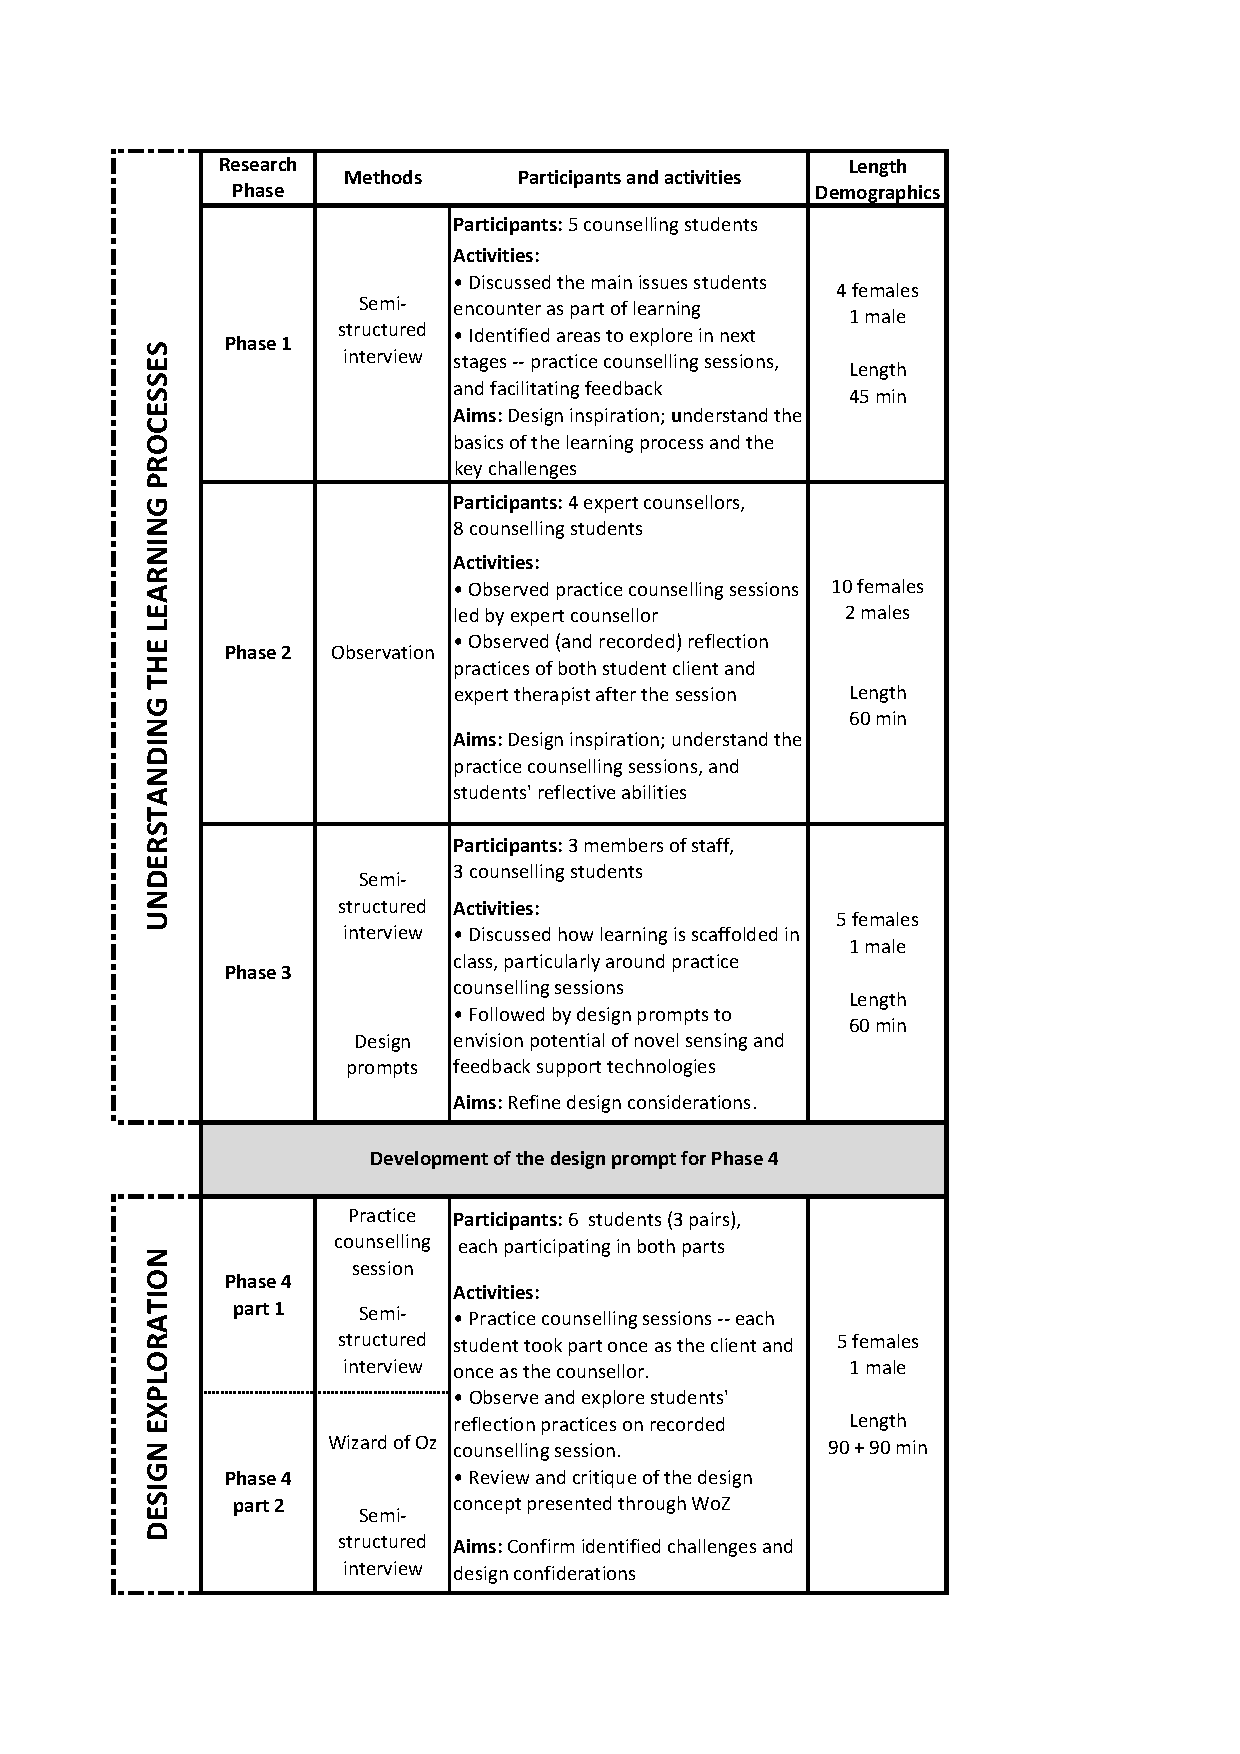
\includegraphics[width=.85\columnwidth]{images/Method-table.pdf}
	\caption{Outline of the iterative design approach -- methods and activities for each phase}
	\label{fig:MethodsOutline}
\end{table}

However, there is very limited work looking at students' actual learning experiences, as opposed to studies measuring `objective' outcomes of training programs (such as ratio of open/closed questions). Similarly, very little is known about the key challenges for learning interpersonal skills as perceived by students \cite{Bulpitt2005,Hill2007a}, or how technology solutions could be mobilized to support student learning in this regard. 


\subsection{Technology and interpersonal training in other settings}
A large body of work in CSCW and HCI has recently focused on technology support for social skills training for disadvantaged populations. Most of this work has supported people with autism spectrum disorders (see review by Kientz et.~al.~\cite{Kientz2013}), and in particular on children with autism with a view to supporting aspects such as basic collaboration (e.g., \cite{Piper2006}), core interpersonal acts such as eye-contact or turn taking (e.g., MOSOCO \cite{Escobedo2012}), or self-reliance (e.g., \cite{Hong2012}). Outside of the autism domain, researchers have looked at using Virtual Reality systems to support the training of people with anxieties such as Social Phobia (e.g., in \cite{Klinger2005}), or video-based training of interpersonal skills for parents of children with behavior problems \cite{Kennedy2011}. 


In contrast, design and research in HCI on the teaching and learning of interpersonal skills for non-challenged populations has so far received only limited attention. Existing work includes, for example, the early exploration of opportunities offered by virtual agents to augment the training of communication skills for medical students \cite{Johnsen2007}, inter-cultural communication training for US Army soldiers \cite{Core2006}, and automated system to improve non-verbal behavior during work interviews \cite{Hoque2013}. 

However, none of these systems embrace the full complexity and mastery of interpersonal skills---such as picking up on subtle feelings and thoughts that might be hidden to the client himself---that are needed and developed within counselling settings.

%%%%% ADD THE TABLE 1 HERE!! %%%


\section{Approach (Method \& Procedure)}
This paper presents findings from a series of interviews and observations that form part of an ongoing collaboration with a counselling degree program in the UK. We aimed to understand how interpersonal skills were taught and scaffolded in counselling training, and the challenges that this may entail generally and for technology design more specifically. We took an iterative, four phase research approach, with each of the stages being analyzed and informing the next (see Table~\ref{fig:MethodsOutline} and below for more details). Overall, 3 teaching staff, 4 expert counsellors and 19 counselling students took part in the various research activities\footnote{Altogether 22 females and 4 males participated. This reflects the ratio of females to males in the course. Generally, each participant took part in a single Phase only; with the exception of three students participating in two Phases each.}. We also drew on our multi-disciplinary research team, comprising a counsellor, interaction designer, psychologist and computer scientists. 


\subsubsection{Phases 1-3: Understanding the design context} 	
In the first phase, we conducted 5 semi-structured, 45 min long interviews with 5 counselling students to explore how they experienced their skills training with a particular focus on their difficulties for learning.  Based on these interviews, we identified that so called `practice counselling sessions' formed an integral, but also the most challenging part in their learning. 

In the next, second phase, we thus aimed to gain insights into some of the practical issues that surround `practice counselling sessions', and to increase our understanding as to how expert counsellors and students reflect on these sessions afterwards. We  observed a set of eight practice counselling sessions that involved overall eight students and four expert counsellors (approx. 20 min for each session and 40 min for reflection). Our analysis of these initial two phases led to first ideas for a potential technology design that centered on the development of an online tool to provide students with a wide range of opportunities to reflect, annotate, and receive peer feedback on practice counselling sessions. However, we were not certain which of these might be most relevant and useful for the students, and how these would fit the existing learning processes.

The third phase therefore aimed to elicit critique and comments on our initial ideas, and to gain a better understanding of how such a technology solution would fit into existing learning practices. We conducted semi-structured individual interviews (60 min) with three teaching staff and three master students. Each interview was divided into two parts: During the first, we asked participants to describe their experiences of how counselling skills are taught and practiced, focusing specifically on how students work with recordings of their practice counselling sessions, and their previous experiences of technology use as part of this process. During the second, we then presented our interviewees with a series of design prompts in the form of post cards that visualized different ideas for potential sources for \emph{feedback} (e.g. by tutor vs. other students; opportunities for video annotations; ideas for automatically generated feedback on the interaction dynamic between conversation partners); and offered examples of certain \emph{modalities} for capturing such information (e.g. 1st or 3rd person camera perspective for video recordings; use of a smartphone app vs. physical buttons for providing feedback; use of sensor devices). These cards were used during our conversations to invite discussions as to where, when and to whom this data should be accessible, and also extending our knowledge on some of the specifics of the learning process that were not mentioned previously. 



\subsubsection{Phase 4: Translating identified challenges into design}
Our findings from Phase 3 enabled the refinement of some of our considerations for the design, leading to the development of a low-fidelity design prompt for Phase 4. This fourth phase consisted of interviews exploring the ways in which students reflected on their skills practice in greater depth, and also provided an initial, Wizard of Oz- style testing of our low fidelity prototype. Three pairs of students joined discussion with the researchers, each on two separate days. During the first meeting (90 min), we asked each pair to run two practice counselling sessions with their partner (so that each student took the role of both the client and the counsellor) and then interviewed them separately. As part of the interview, we invited the students to use the video recording of their session to talk us through their usual reflective processes. This led to a set of 6 interviews and 6 practice counselling sessions. For the second meeting (90 min), each student would be individually be invited to discuss their experiences with our design prompt and to share their assumptions and ideas for technology design aimed at supporting their learning process. This phase is described in more detail in the Design Probe Exploration section on p.~8. 


\subsection{Analysis}
All collected data from Phases 1 to 4 underwent a two-stage analysis process, whereby the data of each phase was at first analysed individually (to inform preparations for subsequent phases), and then revisited as a whole once the data collection was completed. Our final data set therefore encompasses all audio-recorded interviews which were transcribed, and then included into a systematical thematic analysis following the approach by  \cite{Braun2006}. To this end, two of the researchers closely familiarized themselves with the data to identify and systematically search for (reoccurring) themes. Identified themes were then coded and higher-level categories developed. Our findings present the key themes that evolved through this analysis. To protect anonymity, participants are referred to using an abbreviation of their role such as a T for teaching staff or S for student, followed by a participant number.
% }}}


% {{{ SECTION: Understanding the learning process
\section{Part 1: UNDERSTANDING THE LEARNING PROCESSES}
This section presents our findings around the current teaching processes that mediate learning of interpersonal skills for student counsellors, building mainly on the data gained from Phases~1-3. We start by outlining the fundamental approaches shaping counsellors' learning, and then focus on reflection practices around the practice counselling sessions. 

\pagebreak
\subsection{Fundamental learning practices}
Our interviews with staff and students highlighted several core learning practices that were used throughout the counselors' learning. We first discuss the underlying values that shape the overall learning approach. We then outline the learning stages that students undergo, with a specific focus on the practice counselling sessions that were presented to us as the main vehicle for the learning of interpersonal skills.

\subsubsection{Experiential, non-directive learning}
Both students and tutors understand the learning process as (a) fundamentally based on tutors' on-going modelling of counselling skills (e.g. being empathic, congruent, respectful to other's experiences) in all their interactions with the students; and (b) strongly shaped by person-centered counselling values of \emph{non-directiveness}, \emph{experiential learning}, and a \emph{focus on here and now}. In particular, both students and tutors referred to the non-directive approach, describing its evolution from a core belief that people learn best if they feel they are understood and that their perspectives are valued by others; rather than simply being told what to do. As such, the learning processes were described by teaching staff as designed to help students directly experience what they learn about, and to deeply engage with and reach new insights about themselves through reflection -- helping them to \qq{}{push the edge of their awareness} (T1). As such, counselling skills are learned: \qq{}{through creating an experiential classroom in which they can always be working on themselves. So no role play, no pretending to be anybody else, just really working on their authenticity, presence, their capacity to engage with themselves, intra-personally, and interpersonally} (T2).


\subsubsection{Discomfort as a cue for learning}
In addition, teaching staff regarded experiential learning to only happen when students are \qq{}{willing to come out of their comfort zone} (T2). This is particularly important due to their belief that, if one is to learn, \qq{}{there needs to be a dynamic moment of feeling off-balance, like a waking up moment. Then you have to realign yourself and in that process of realigning I think you learn} (T2). This highlights the need for enabling, at least to a certain extent, rather uncomfortable experiences to invite important processes of reflection and thereby the development of interpersonal skills. However, the teaching staff as well as the students frequently emphasized how such interactions had to be facilitated within a 'safe space', where confidence and trust could develop among the students (and the staff). This need for a safe space and mutual respect was also manifested in a 'learning contract' that all students and tutors agreed to, and whose breach would be severely reprimanded. 

\enlargethispage{\baselineskip}
\subsubsection{Learning in stages}
Tutors described how they structured activities across the study program to stage the learning of counselling skills. Their goal entailed that students started their training by developing deep self-awareness and reflection abilities, scaffolded for example through sessions that aimed to support students to re-live strong feelings (e.g., shame, loneliness, loss). This was followed by rehearsing core interpersonal skills such as attentive listening, understanding or paraphrasing the other, deliberately practicing  each in 'isolation', without being connected to other aspects of the interaction. Only then the students would move onto the key part of the training---practice counselling sessions---where the interpersonal aspects of counselling skills were developed, tried out, and fine-tuned before the students were able to embark on interactions with real clients as part of post-training placement. 

\emph{Practice counselling sessions:} \quad Practice counselling sessions were described as the crucial stage where interpersonal counselling skills are taught in context. Such sessions took place in a `triad', where three students took on the role of a `client', `counsellor' or `observer'. During the practice sessions, the student in the role of the `client' was encouraged to talk about a real issue -- one that felt important to them and that was not too sensitive to be discussed with the student learner in the role of the counsellor. Frequently however, students reported how `clients' would bring quite intimate topics to these sessions, such as substance abuse in the family or serious marital and relationship issues. 

Participants explained how such practice sessions would be scheduled regularly (e.g., weekly) and that the sessions last between 5-20 minutes, with the duration increasing over time as students' experience with the activity develops. Each session is usually followed by a feedback phase (around 10 minutes long), where the observer, and, at times, also the client or counsellor, would share what they had observed during the interaction. Occasionally, the tutors would join the triad as additional observers and providers of feedback. Moreover, the students commonly rotated in the roles they were taking, enabling each to practice their counselling skills in turn. Some of these triad sessions were further reported to have been video recorded (e.g. 3 to 4 sessions a year) but there were no other reported uses of technology. 

The key part of the learning was however described to occur \emph{after} the practice session had finished, when the counselling student would `process' and reflect on their experiences. Supporting students in their reflection and processing of their practice sessions was therefore regarded as vital for interpersonal skills learning. 

\subsection{Learning through interpersonal reflection}
We now describe in more detail how students engage with such post-session reflection work around the practice counselling sessions. We highlight how the focus on the dynamics of interpersonal skill was found to lead to a complex interplay between several types of reflection, complementing a deep personal reflection on students' own experiences from the session with the need for `interpersonal reflection' that draws on shared sense-making with others.

We saw three ways in which such reflection work on a practice counselling session was currently scaffolded: (i) students received \emph{external cues} provided directly after the triad session; (ii) such feedback was then employed to support \emph{self-cued reflection}, when the student reflected on their session repeatedly over time, often at home and alone; and (iii) reflection on selected sessions could be guided through \emph{Interpersonal Process Recall}, which is a structured process to facilitate deep self-awareness of the counsellor. Each is described in more detail below.

\subsubsection{External cues for counsellors' reflection}
Students in the counsellor role highly valued receiving multiple perspectives on their practice sessions, even if these conflicted with their own perspective. They believed there was no `right' interpretation or perspective on what was happening, and such external feedback served as a valuable cue for reflection. 

Both tutors and students described how the observer(s) provide most after-session feedback. Observers are asked to provide a specific kind of comments that are tightly bound to what was directly \qq{}{observed and seen in practice sessions} (T1). Tutor 3 has eloquently described it as 'noticing', saying that \qq{}{I don't want them to make a judgement about whether it's right, wrong, helpful, unhelpful, but just noticing.} However, students told us they frequently struggle with providing such non-judgemental, yet constructive feedback. They particularly struggle with grounding their comments in particular observations. For example, Tutor 3 described how students \qq{}{find it really difficult to be concrete. When I'm doing it I would say, `I notice you asked five questions in a row', full stop.  Whereas a student will often go: `You asked too many questions', and that's a value [judgement]}. Overall, the tutors consider the ability to give good, constructive feedback as an important part of students learning, as well as a method of assessing their development.

\enlargethispage{\baselineskip}
Participants highlighted the qualitative difference between feedback from the tutors and peers. For example, Tutor 1 explains how the tutors are better able to help students pin-point areas for future development---an example of constructive feedback---as opposed to students comments being less useful \qq{}{I think for the tutors, we're more skilled in noticing, [things like] you're really skilled in that area [but] we need really to bring `this' area up [\dots] rather than, `Well, you were very good at this and I liked how you did that and…' Which is kind of generally how it starts off for the students in the second year.} Students viewed this similarly and often were not entirely happy with the feedback they tended to receive from peers, particularly with the lack of critical but constructive comments. For example Student 1 told us that \qq{Lily}{I hate it when people go, `That was excellent. That was great. I loved that.' [\dots] Even if it is genuine, I still hate it because I am not getting anything out of it. I would much rather if someone goes, `Oh, well, I thought that was really good, but maybe \dots'}

Clients can provide very different feedback than the observers, by the nature of their involvement in the session. In fact, their view was considered even \qq{}{more important because they're the one that is experiencing it in the moment, we [the observers] are not. We're just on the periphery as it were} (S1). Students told us they also value clients' feedback highly, as \qq{}{at the end of the day, counseling is all about the relationship with the client} (S12), and especially as \qq{}{in training, when you're not experienced, you don't know what the client's experience is so yes, you've got to know.  So absolutely you need to know how they experienced you.} (S3). However, it is currently not very common for clients to share feedback after the session; and even if they do, it is often only a very high-level overview summary of the session. 

\subsubsection{Self-cued reflection}
Students told us they repeatedly reflect on their practice sessions at home, especially if those were video-recorded. Both students and tutors saw the usefulness of such repeated, deep immersion into the session on video.  As Tutor 1 described, the students would take the video home and \qq{}{every time they watch it they get more and more out of it. [\dots]  So then they'll go away and watch themselves and really, really unpick it.} Similarly the students saw it as an opportunity to \qq{}{work deeply when you see the tape again and again by yourself because I was working my incompetencies and the way I really wanted to improve myself.} (S6) 

We provide a longer example of such a reflective account, taken from the first part of Stage 4, to highlight the depth of reflection students are capable of, as well as to illustrate the various aspects students generally paid most attention to. 
\begin{quotation}
{\itshape
\noindent 
(S15): ``I noticed that when she was talking about handing in her MA [\dots] she said, `That's a really amazing achievement', and there was just like a pause and the slight forcing of her saying she'd had an amazing achievement. In the past I would have been like, `Ah, I noticed that she did that' but [now] I wouldn't want to challenge because I didn't know whether I had got it right, and also I didn't want to stop her flowing. So I held on to that and she talked for a little while and then I found a pause and was able to say, `I noticed that you did this. I just wanted to know if you noticed anything?' Then she thought about it and talked it though, and it turned out that she had some difficulty accepting that she'd had an achievement, because of various things that were to do with the support of her husband and stuff. \smallskip	

\noindent Interviewer: How does that make you feel?	\smallskip

\noindent (S15): Really good. It gave her the option to change the flow of what she was talking about, to get a little bit deeper into acknowledging her own feelings, which is really important. So that's really good. I was really authentic [\dots] I noticed how I felt, [and said] `I noticed something there. Did you notice?' So that was really good. Well done me.
}
\end{quotation} 

The example illustrates how students generally paid attention to several interrelated aspects. First, we see a very detailed focus on their own and the client's non-verbal behaviour. While non-verbal behaviour is important also during the session, students often picked up on cues they have not noticed before revisiting the video. As S12 says, 	


\begin{quotation}
{\itshape
\noindent 
(S12): You still spot things the third or fourth time that you hadn't spotted, perhaps, the first or second time. Again, with me, it was all about concentrating, again, on not what was said, but what I was doing, my reactions, what were the client's reactions, facial expressions. I thought they are very, very interesting to watch because a smile in the right place, or a frown, or a `Mmm, mmm.' If the client goes, `Mmm,' does that mean they are not quite understanding what I am asking, or saying?'' 
}
\end{quotation} 

Second, the focus on non-verbals was then combined with attempts to go beyond of what the client has said, and create a deeper understanding/interpretation of why they did what they did. For example, S15 has picked up on his client's subtle hesitations around accepting an achievement and used this to uncover a deeper issue they then spend the session talking about. Similarly, most of the students were using the video to continuously analyse and double-check if they had understood their clients well enough during the session; or if they had missed something crucial. Students always view their interpretations as tentative accounts of clients' experience that need to be verified. Such verification is however not a part of the current training processes.

Third, although noticing new aspects can be perceived as validation/clarification with advanced students when they watch the video (e.g., S15 or S12), it can also raise self-critical attitudes. This was particularly common for early students, as the video highlighted things they believed they had missed, or their own responses they thought they could improve. For example, speaking about the bachelor students, Tutor 3 said \qq{}{[T]hey always choose the worst bits and then beat themselves up. They never choose the bits that they do really well and show you that. They always choose the bits where it's all gone, awry. Their own feedback is always more negative than ours, always, both in skills and on written work.} Balancing such self-critical attitudes seemed to be another important challenge for the students. 

Fourth, counsellors often explored alternative ways of responding to a situation in their minds, especially after identifying a situation they were not happy with. Again, these require them to work with complex assumptions about the clients' possible responses and thoughts, but are not sense-checked with the client later.


\enlargethispage{\baselineskip}
\subsubsection{`Interpersonal Process Recall' (IPR) -- guided reflection}
Students are also taught a structured way of reflection, called Interpersonal Process Recall (IPR), as part of their normal learning process. IPR is a traditional technique developed by Kagan \cite{kagan1969} in the 1970s, aiming to facilitate counsellors' deep reflection on, and awareness of, their own feelings and thoughts during counselling sessions -- i.e., the focus is on their own self-awareness and experience of the sessions, not on the dynamic of the interaction as such. A brief description of the IPR process is below, see \cite{Kagan1984} for more detail. 

IPR draws on the collaborative viewing of a video recording of the session. The counsellor can stop the video at any time of their choice, often when they believe something important has happened. Another student or a tutor then asks the counsellor a question from a list compiled by Kagan. The counsellor then uses this to reflect aloud on what was going on for them at that time. If done according to the guidelines, this is a very long process -- e.g., 8 hours of IPR for 1 hour of the videotaped session. As this protocol was originally designed for analysing real-world counselling sessions, the client's view is not supposed to be shared, nor can the clients stop the video at moments they would like to discuss, although they might be present at the IPR session. However, the students saw this as overly restrictive.
%
In fact, students told us that for most of the sessions they facilitated (i.e., without the tutor present), the comments would be eventually shared by all involved. The tutors were aware and accepted that such adaptations of the IPR protocol happen. Moreover, they indicated that they would be open to modify IPR such that would also involve the client to a larger extent; highlighting again the need for more detailed input from the client that is lacking in existing practice. 


\enlargethispage{\baselineskip}
\subsection{Effects of video-recording on reflection practices}
The inclusion of the video recording markedly changes the perception of the practice sessions for the students. Tutors and students agree that having the video is useful as it provides more opportunities to explore and reflect on their own practice in detail, regardless whether it was to support external cues, the students' own reflection at home, or IPR. Video is understood as providing `evidence' and specificity to reflection. In other words, by having the option to stop and point out particular moments, it was perceived as helping provide specific, non-judgemental grounds for deep reflection on the part of the student counsellor. 

While the students saw the video as beneficial for their learning process, students also told us that they initially felt conscious, vulnerable, and very uncomfortable about the video recording, although they eventually get used to it. Tutors were aware of these challenges for students, but believed that this is an important part of the learning process, and that the benefits outweigh any uncomfortableness whilst doing it. For example, after giving an example of her own experience with video-recorded skills practice (as a student), Tutor 2 told us: \qq{}{As soon as you start to get the feedback and you begin to see, `Oh my God, this is powerful. I'm really learning a lot about myself here', the equipment becomes an aid not an enemy}. 

Video-recording also raises pragmatic concerns that hinder its use for all sessions, as it takes longer to set up, and \qq{}{if you're doing short sessions it's not feasible} (T3). However, tutors are keen to extend the use, and have for example already started including it into bachelors course, with good uptake from the students. For example, Tutor 1 described her experience with using video for second year BA students who \qq{}{enjoyed it when they did it. Yes. Terrified of it, of course (…) they really did get the benefits of it.}


% }}}

% {{{ SECTION: Identified Challenges to Learning and Design
\section{Part 2: CHALLENGES TO LEARNING AND DESIGN}
While the practices around the teaching and learning of counseling skills are effective, to the extent that students graduate as counselors, there are also a number of challenges that can point to opportunities for technology support. We first highlight the key challenges to learning we identified from the Phases 1-3 of our data collection. We then draw out four design considerations for systems aiming to support counselling learning that build on the identified challenges, and outline how these considerations guided the design of the design prompt we used for the Phase 4. 

\subsection{Summarising challenges to learning}
We saw that counselling skills are taught and learned through mostly an experiential learning process, with marked emphasis on students' reflective practices. The deep awareness of own feelings, thoughts and experiences is considered as the key precondition to successful learning of counselling skills. However, the crucial part of the learning takes this a step further: to a reflection on, and an awareness of, the interaction and dynamic interchange between the counsellor and client -- i.e., interpersonal reflection. 

The key aspect in counsellors' counselling skills development is thus a complex reflection process by which students aim to deeply understand how their own actions have affected the client's thoughts and feelings; yet, these might not be directly observable and would need to be collaboratively established. However, the existing scaffolding of students' reflection mainly focuses on supporting reflection on the student-counsellors' own internal processes, and only marginally facilitates the focus on the `client' or on the dynamics of the counselling session. We list key issues with supporting such interpersonal reflection we identified in the reflective practices we observed and discussed with participants:

\emph{External cues for counsellor's reflection:}\\
External cues for reflection can come from clients and observers. However, clients' feedback is rarely elicited, despite the fact that it is felt by students as more relevant than the one from observers; and even when it is given, it is provided in a high-level, summary way and lacks specificity. Participants also emphasised how providing good, constructive feedback from the observers' position is a difficult skill to learn. The students are often not satisfied with the feedback quality they receive from their peers; but also with the quality of feedback they are able to provide themselves when in the role. Similarly to the feedback from clients, our data suggest again a lack of specificity in the `noticing' feedback. This is possibly due to the limited time available, usually just a 10 minutes long period, and the lack of support to provide localised feedback, such as the ability to point back to specific moments in a video recording for the observers.  

\enlargethispage{\baselineskip}
\emph{Self-cued reflection:}\\
Self-cued reflection is also an important part of the learning process. However, students described how there is a very limited support for further interaction with the client and observers, although the inferences about the others' thoughts and feelings are crucial for students' reflective processes in this stage. This makes it very difficult to check whether counsellors' own assumptions and expectations of the client and observers' experiences are correct. 

Moreover, students' reflection practices at home lack scaffolding or structure, and students resort to waiting for interesting moments to `pop-up' when they are watching their session on video. This is not because the students would have trouble reflecting as such, as we saw how students are able to produce very detailed and `thick' accounts of their own experience, intertwined with their interpretations of what the client likely felt/thought at that particular moment. Instead, we argue that it is exactly this ability for nuanced reflection, together with the lack of cues to help direct attention, that leads the students to pay attention to too many things at once.

\emph{IPR -- guided reflection:}\\
The IPR process provides an inherent structure that seemed to support a better focus and the deepening of reflection for students. While this suggests that similar approaches to scaffolding reflection might be useful also for the other reflective practices (such as external feedback and self-cued reflection), the IPR however does not directly support interpersonal reflection. Instead, it focusses on the self-reflection of the counsellor only, with little input from the client or observers, and brings extreme time requirements for all involved. 

\subsection{Design considerations to support counselling training}
Each of the three key reflective practices highlights particular facets that are crucial for interpersonal reflection, but each is, for pragmatic reasons, used independently in the current learning process. This points to opportunities for technology to combine and support all of these aspects of interpersonal reflection together, as well as to address some of the key challenges present. 

In particular, the importance of external cues highlighted the need to include the client and observers in the interpersonal reflection process of the student-counsellor. Self-cued reflection then highlights how counselling students process and learn from their practice sessions over longer periods of time, and thus do so mostly outside of formal learning settings, e.g., at home. The IPR then suggests the benefits of scaffolding reflection non-directively, i.e., providing structure for reflection but keeping the student-counsellor in charge to decide what to focus on and when; and also pointing to the importance of specificity and `evidence' that a video recording can provide. We now outline four design considerations for systems aiming to support counsellors learning in similar contexts. 

{\bf (C1) Non-directive facilitation of the reflection process:}\quad We already brought attention to the limited scaffolding for interpersonal reflection processes, especially for the counsellors' self-cued reflection outside of the lessons. Technology supporting such reflection should empower students to reflect and make personal choices, rather than directively restrict their experience. Furthermore, designs should aim to facilitate localised reflection, i.e., tying the reflection and feedback to particular moments of the session to provide specificity and `evidence'. 

{\bf (C2) Support co-constructing of interpretation with the client:}\quad We saw the need for processes or technologies that facilitate a better access to clients' experiences for the student in the role of the counsellor during their reflection process. In particular, technology should facilitate interactions with clients (and observers) to allow counsellors to verify and sense-check the intricate assumptions they may make about their client's feelings, thoughts or behaviours. Further facilitation would be useful to support students in making their reflection work or felt experience more tangible, and thus more suitable for discussion. 

{\bf (C3) Scaffold constructive feedback from observers:}\quad Providing constructive feedback from the role of an observer (or client) is understood as an important but difficult skill that students need to learn but tend to struggle with. In particular, students find it difficult to be concrete enough and link their comments to specific observations; or to provide constructive criticism instead of praise. Technology should aim to facilitate such localised, constructive (i.e., not only positive), but still non-shaming feedback from the observers, as well as support the observer's learning whilst giving feedback, e.g., scaffolding it as a valuable self-reflection exercise. 

{\bf (C4) Support for iterative, multi-phase reflection:}\\ Our data suggests that interpersonal reflection requires a long-term process, combining periods of deep individual sense-making and reflection (including creating assumptions about others' experiences and states), with periods of interactions where such thoughts are shared, checked and discussed. Technology should aim to scaffold such a series of in-depth engagements between the client, the counsellor and the observers, including enough time for deep reflection in between. It is also important to respect and design for the limited time available for the students (as opposed to a full IPR process).   

\enlargethispage{\baselineskip}
\subsection{Developing a design prompt: The AffectDial}
To design a design prompt for use in Phase 4, we drew on the identified design considerations above, and recognized the value of the video as a data source for reflection. In the scope of this paper, we only focus on one of a series of design prompts that were employed with participants: the AffectDial, as it explores possible design directions to many of our design considerations (C1, C2, C4).
%Due to space constraints, we do not outline the full design concept of the probe in this paper\footnote{The full design probe is based around students' use of video for reflection and framed as an online tool that allows the students (and tutors) to interact with each other and analyse the video-recording of their session through a browser interface. We suggested various functionalities to scaffold, and share, reflection on different facets of each persons' experiences (non-verbal behaviour, emotions etc.).}. We instead focus primarily on a specific part, called  Our choice of AffectDial as the key focus here was motivated by the fact that it 
%
The AffectDial is an interactive mock-up prototype that takes the form of a virtual `slider' on a single line with two poles, where poles can represent any concept that students wish to explore, e.g., from non-empathic to empathic. The student can indicate their in-the-moment experience while they watch a video-recording of their session, by manipulating the slider position by moving the mouse. The sequence of such slider position changes is recorded, time-stamped to tie the changes to the respective time in the video, and can be thus later presented as an overview graph (see Fig.~\ref{fig:affectDial}). 

We envisioned that uses of the AffectDial would support novel reflection practices for the students in several ways. First, asking students to choose a specific concept to analyse could help them prioritise and make conscious decisions about which aspects of their counselling skills they want to specifically focus on. Moreover, we expected AffectDial to promote sustained attention, as the slider position is to be continuously changed according to felt experience. Visualisation of the resulting trace once it has been indicated could further support localised reflection, as it is tied to the video-recording. Altogether, AffectDial was therefore expected to non-directively promote focussed reflection (C1). 

Second, we also envisioned that AffectDial could directly promote students' perspective taking and help explore the differences in experiences between client and counsellor. For example, the student can decide to use AffectDial to indicate not their own experience, but their assumptions about how another person feels -- e.g., we asked the students in the role of the counsellor to indicate how they believe their client felt as part of Phase 4. Moreover, once such a AffectDial trace is created, it can easily be presented to the client for comments, or compared with the client's own AffectDial trace of the same concept, making it a tangible visualisation of the reflective process. Finally, the time required to provide feedback with AffectDial equals only to the time needed to watch the part of the session to be rated. This is quite time efficient, especially when compared to IPR or similar procedures, and could allow for iterative engagements. As such, we hoped that interaction with the AffectDial would promote co-construction of interpretation through sharing and discussion of felt experiences with the client (C2), and do so by facilitating an iterative, multi-phase engagement with the data (C4).
% }}}

\begin{figure}
  \centering
	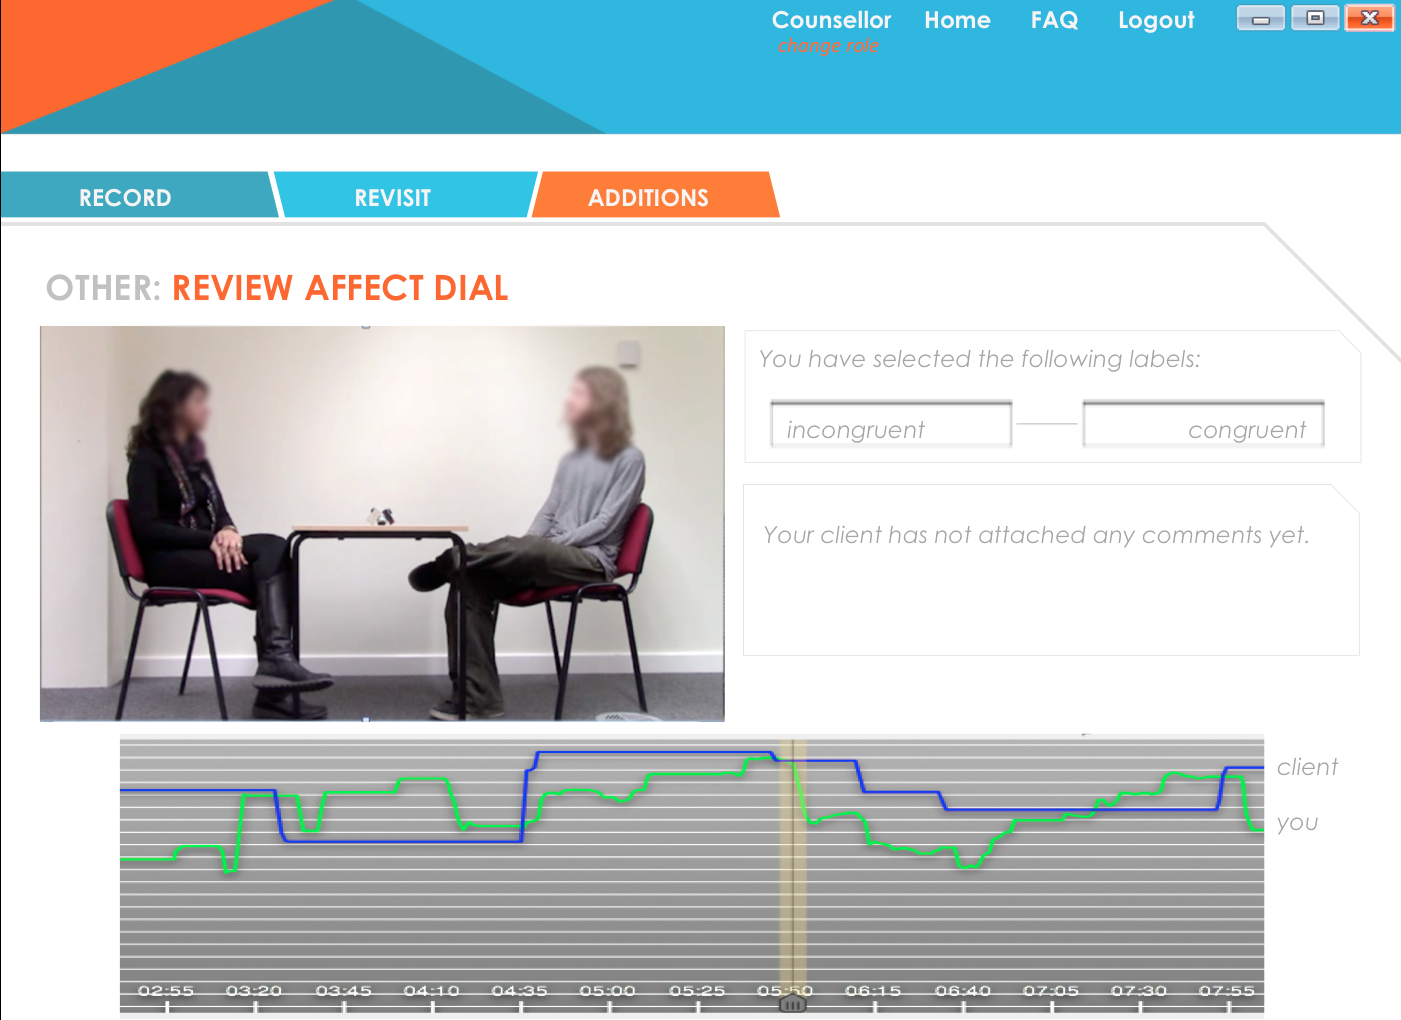
\includegraphics[width=.95\columnwidth]{images/AffectDial.png}
	\caption{Visualisation of the AffectDial traces, connected with the video, as presented during the Wizard of Oz (Phase 4).}
	\label{fig:affectDial}
\end{figure}


\enlargethispage{\baselineskip}
% {{{ SECTION: Design probe exploration
\section{Part 3: DESIGN-LED EXPLORATION}
\label{sec:Probe}
In Phase 4 of our research process, participants were invited to explore the AffectDial. Following their engagement in a practice counselling session, we first let the participants explore the AffectDial in conjunction with their video recording and to discuss their experiences with one of the researchers. We then explained and guided participants through available as well as envisioned functionalities of this design prompt, asking for their thoughts and input. 

%Phase 4 explored participants' responses to this design probe, presented through a Wizard of Oz (WoZ) process. Our key goal was to further explore and check our understanding of the identified challenges and the possible design directions, rather than to pilot a designed system.

%The design probe was presented as a power-point mock up of an online system, complemented with a software package developed to collect the AffectDial data. The presentation was personalised for each participant by including the videos from their practice counselling session, which was run in the first part of Stage 4. During the WoZ, we first let the participants test the AffectDial, explore the resulting data, and discuss their experiences. We then went through the rest of the functionalities  of the full design probe step-by-step, asking the participants to envision if and how they would use such options. The overall feedback on the full probe was largely positive (as also exemplified by the AffectDial discussion below), including valuable suggestions for how to evolve the design further. However, due to space constraints, it is beyond the scope of this paper to discuss these more fully here; and we focus on the AffectDial interaction in detail instead. 
%
% Ger: Could just give the overall feedback eg that people largely positive and also had some good suggestions for how to evolve the idea but beyond scope to discuss any more fully here... or go into affectdial as the detail
% from v2:  Overall, we received very positive feedback on both envisioned usefulness as well as the fit with existing learning processes; as also exemplified by discussion of Affect Dial below. 
%
%We return to the implications of these findings for the design considerations in the Discussions section.
%
%\subsection{AffectDial interaction}

We prepared a specific sequence of interactions with the AffectDial that we asked students to do. These aimed to explore the combination of explicit perspective taking (i.e., counsellor indicating their assumptions about client's experience) and facilitated sharing of experience between the student-client and counsellor via the Affect Dial trace.  

In particular, we first asked the counsellor to decide on a concept they would like to ask their client to feedback on with the AffectDial (e.g., how anxious the client felt). The counsellor also chose a 5-10 minute long fragment from the session they've just finished, to specify which part of the session the client was asked to watch and thus give feedback on. We then passed this information to the client, who was in a different room, and who used the AffectDial to indicate their experiences regarding the chosen concept on that fragment. Independently, the counsellor rated the same fragment and concept, but \emph{from the perspective of the client}, e.g., indicating how anxious he/she thinks the client was at moment. The two traces were thus recorded independently, but when brought together, this allowed the counsellor to compare the AffectDial trace visualising their own assumptions of how, e.g.,  anxious the client was, with the trace indicating the felt anxiety directly by the client.  

We then presented the counsellor with the overview of both AffectDial traces and let the counsellor explore and compare these. The traces were connected to the video recording and counsellors could easily move to and review moments in the session they found interesting (see Fig 1). We recorded such interaction with the AffectDial for each of the six practice counselling sessions in Phase 4. The following presents the findings from this process.

%the students' interaction and responses around the AffectDial reflection tool. 

\subsection{Students' responses to the AffectDial}
All six students found the slider interaction understandable, and were able to decide upon a concept they would like their client to feedback on. The chosen concepts ranged from selecting one of the core Rogers' conditions such as felt empathy or congruence, to more specific concepts such as `positively to negatively challenged' or `helpful to unhelpful facilitation'. 

Students shared with us that---by limiting their attention to a single facet of the experience and continuous manipulation with the slider---the interaction with the AffectDial often facilitated a state of heightened awareness just for behaviours around the selected concept (without distraction by other aspects). This was described as a novel and pleasant experience for many students. For example, S15, who was indicating `challenging responses', explained: \qq{Ben}{I'm not really focussing on any of that [other aspects], I'm just focussing on the flow into whether I'm going to challenge or not and when there's a right pause, or whether I've missed it. That's quite interesting, just to go through that experience and be so focussed. [\dots] Because it's [usually] so heady, it's so cerebral and sometimes overwhelming, it's not something that I've really experienced, the breaking down into just one aspect. To do that was quite refreshing.}

Importantly, comparing their own and the client's trace helped students identify very specific moments they wanted to explore further. These were particularly moments where the two traces did not match (e.g., the client indicated a sharp position change of the slider while the counsellor did not) and thus the counsellor felt to may have misunderstood the client. Once the students returned to such moments (by re-watching the relevant part of the video), we saw them often re-frame their previous understanding of the situation. For example, S11 asked to revisit a particular fragment where her client indicated a drop in perceived helpfulness, but S11 did not. After revisiting the video, she shared: \qq{Carolyn}{I think what happened there is [that] all I did then in my response was just copy, paraphrase of what she said, but that's it; I didn't do anything with it, I just reflected it. I think [she] needed a little bit more of something from me. [\dots] If I'd just watched that back, I wouldn't have picked that up.} 

Students also often suggested that, as a next step, such pinpointed moments and the re-framing they made are something they would have liked to take further and discuss with their client face-to-face. In other cases, for example when the traces did match remarkably, this served our students as a useful validation, i.e., that the assumptions they had were consistent with what the client experienced -- which is something the students said they didn't have access to before. Similarly, the overview mode at times highlighted particular moments to look at for the counsellors even before seeing client's data, i.e., the overview showed some aspects they were not aware of when doing the reflection-in-the-moment.

Although the AffectDial functionality generally received a very positive response, students highlighted concerns related to potentially hurting the feelings of the counsellor after the feedback is exchanged, e.g., if the client was to indicate they perceived no empathy in a particular moment. While no such occasion arose during the six interactions we recorded, there is a clear need to ensure mechanisms are in place to safeguard practice; such as the opportunity to discuss the indicated traces in person soon after exchanging and/or opportunity to provide more detailed written explanations for parts that might perceived as hurtful. 


% }}}

% {{{ SECTION: Discussion
\section{DISCUSSION}
Learning how to develop sophisticated interpersonal skills is a critical but challenging part of studying to be a counselor. Participants in our studies painted a nuanced picture of their learning processes, and the importance of interpersonal reflection practices to learn counselling skills. In this section, we discuss how these findings might inform the design of systems to support learning of interpersonal skills in the counselling setting. 


% {{{ Specifics of interpersonal reflection 
\subsection{Specifics of `interpersonal reflection' in counselling}
Our findings show how learning of interpersonal skills in counselling is an inherently social endeavour, building on a complex interplay of interpersonal reflection processes around practice counselling sessions, and involving multiple actors. In other words, we saw that although the student in the role of a counsellor might do most of the reflection work, the reflection process cannot be fully completed by any one participant alone. The client and possibly observer(s) need to partake and share their perspectives to jointly co-construct the interpretation of the session, and this is needed for the learning to take place. As such, the focus on the `interpersonal' comes in several variants -- the activity itself, the skills that are learned and thus reflected on, and the interactions between the counsellor, the client, and observers in the processing stage after the practice session. As highlighted by the suggested design considerations, systems aiming to facilitate counselling learning will need to take into account, and provide support for, all these aspects of interpersonal reflection.

This presents an interesting reflection case that is complementary to  existing reflection research in CSCW and HCI. The majority of such work aims to cue or facilitate reflection on individuals' reflection (e.g., \cite{Sas2011,Stahl2008,Thieme2011,Isaacs2013}) supporting people to become more thoughtful about their everyday experiences. In contrast, the understanding of reflective processes as a collaborative social activity is relatively rare \cite{Fleck2012,Prilla2012}, and is arguably an area ripe for more detailed study \cite{Baumer2014}. Further exploration of the interpersonal reflection processes, which we saw as crucial for counsellors' learning, could thus contribute to this increasing interest to explore technology support for social reflection, as a relevant part of learning and sense-making in other social situations.
% }}}

% {{{ Returning to design considerations 
\subsection{Returning to the design consideration} 
Building on our experiences across the Phases 1-3 of this research project, we drew out four design considerations to support interpersonal reflection, which were then further explored in Phase 4 with a design prompt. We now return to these considerations to discuss the broader implications and opportunities for technology, using the experiences with AffectDial to ground our observations. 

\subsubsection{Non-directive facilitation of the reflection process}
One promising option to non-directive facilitation is to support the learner in focusing their attention to specific aspects of the interaction. For example, the structure `enforced' by AffectDial---i.e., the need to choose and focus on a single concept while watching the video---led to very deep and focused reflection, while keeping control over the content in the hands of the counsellor.  Similarly, the ability of technology to allow for easy re-structuring and novel viewpoints on data, such as the real-time indication combined with a post-hoc overview, can further support a focussed reflection process. 
Moreover, prior HCI work (e.g., \cite{McDuff2012,Stahl2008}) suggest the possibility of using sensor or video-based data to provide people with novel cues for reflection and learning. Such cue-based support could again help to focus attention and empower students to explore novel interpretations of their and others' experiences. In particular, the recent advances in detecting relevant social signals such as non-verbal mimicry \cite{Bilakhia2013,Vinciarelli2012} could be a promising avenue to explore in future work.

\subsubsection{Support co-constructing of interpretation with the client}
We saw that understanding of others' perspectives and feelings is a core aspect of counsellors' learning, but that the counsellor is unable to reach that understanding without including the others into the reflection process; this is an endeavour that often requires large commitments from all involved. As one possible approach, by helping make participants' reflection work or felt experience more tangible, technology could support counsellors in identifying, challenging, and testing their own assumptions about the other's experiences. For example, the perspective taking exercise with the AffectDial not only provided a visible trace of a particular facet of the client's lived experience, but also allowed the counsellor to visualise and directly compare her own understanding of what the client could have been feeling. While such a single slider trace cannot encompass the full complexity of the counselling interaction (a problem likely shared by any technology tool in this space), it still seemed to allow the counselling student to either `validate' their understanding, or pinpoint specific moments where misunderstandings were more likely to occur. Once such specific moments were found, the students used these to improve their understanding of the interaction. Moreover, they  believed such moments could provide good grounding for further discussion, and thus help the counsellor and their client to jointly re-frame their interpretation and understanding of the interaction. 

\subsubsection{Scaffold constructive feedback from observers}
We suggest that technology can help scaffold the 'noticing' process for the observers, supporting them in providing more specific and non-judgemental feedback, but also facilitate the learning of their feedback-giving skills. For example, mobile or wearable technology could be used to help student observers ground their observations to specific moments within the session on-the-fly, such as allowing them to `tag' situations they would like to comment on while observing the session. Not only would this be a useful, grounded feedback for the counsellor, but also the act of tagging such situations could provide material for a more specific reflection and learning on the part of the observer. 

Moreover, the distancing nature of technology, especially when used to provide feedback remotely, could be utilised to facilitate more `honest', constructively critical interaction. For example, we would expect observer feedback given through AffectDial to work this way, as it: (i) asks the observer or client to non-verbally indicate their own personal experience, and as such it is not felt directly as a judgement of the counsellor; and (ii) the act of requesting such information alone includes an implicit `permission giving', as the counsellor is the one to select the concept in question and the part of the session to be looked at. Still, designs using such mechanisms need to put safeguards in place (e.g., allowing the counsellor to give `feedback on feedback' back to the observer) to make sure that the interaction stays constructive, and that any misunderstanding or hard feelings are promptly talked through. 

\subsubsection{Support for iterative, multi-phase reflection}
Asynchronous interaction, such as various forms of focussed `requests for feedback' sent by the counsellor to the client, could prove particularly useful to support the long-term, multi-phase interpersonal reflection process. Such asynchronicity allows the individual students to engage with the sessions at the time of their choice, and provides an opportunity for the counsellor to carefully select the parts of the session they are particularly interested to focus on. We envision that such a series of asynchronous, iterative interactions would help identify a set of key discussion points, leading to a more in-depth and focussed face-to-face engagement to jointly interpret and discuss differences in viewpoints. This is again exemplified in the interaction we staged as a part of such a process with the AffectDial, where the counsellor first reflected to select both the concept they were interested in as well as the part of the session to be looked at by the client. Once the request had been fulfilled (a relatively easy and quick activity for the client), the counsellor received useful data to further guide their own reflection, often leading to a focussed set of points they would like to discuss with the client in more detail at a face-to-face meeting.
% }}}

% {{{ Broader implications
\subsection{Broader implications -- social skills learning}
The lessons from the counselling context can also inform and inspire a broader agenda looking at social and emotional skills learning in other settings, such as training for medical staff \cite{Barth2011,Stepien2006}, leadership \cite{Bono2009}, and increasingly also school education \cite{Durlak2011}. These are all areas where development of interpersonal skills is also crucial, and where similar sets of learning approaches are being used, including experiential learning and the need for interpersonal reflection \cite{Zins2007}. As specific examples, curricula aiming to teaching skills such as empathy, awareness of own and other's emotions, or perspective taking are increasingly rolled out across primary and secondary schools within the US \cite{Durlak2011,Weare2011}. Similarly, there is an established need in the medical community for an increase in support for training communication skills and empathic interaction for medical staff across all roles \cite{Barth2011,Satterfield2007,Stepien2006} -- including students, practicing doctors, and nurses. 

As all these programs use very limited technology so far, this opens questions if and how could CSCW and HCI support the social and emotional learning in these settings, and whether the findings around the opportunities to support counsellors' learning here could serve as a good starting point. 
% }}}


% }}}

% {{{ SECTION: Conclusions
\section{CONCLUSIONS}
This work presents a first exploration into the role digital technology could play in supporting the learning of interpersonal counselling skills. We present a nuanced understanding into how such skills are taught as part of a humanistically oriented counselling degree program, highlighting the challenges to learning students currently face. These revolve mainly around the need to better support interpersonal reflection processes, which are crucial for the student learners. Drawing on our interviews, observations and the design prompt, we offer four design considerations for systems aiming to mediate such challenges. Overall, our findings point to the potential for technology to enhance and support the learning of interpersonal skills in counselling training, and possibly also other settings, and provide an important first step for future research in this direction. 
% }}}










\section{Acknowledgements}
Blank for review  




\bibliographystyle{abbrv} \bibliography{library}





\end{document}


